\documentclass[12pt, twoside]{article}
%\documentclass[12pt, twoside]{article}
\usepackage[letterpaper, margin=1in, headsep=0.2in]{geometry}
\setlength{\headheight}{0.6in}
%\usepackage[english]{babel}
\usepackage[utf8]{inputenc}
\usepackage{microtype}
\usepackage{amsmath}
\usepackage{amssymb}
%\usepackage{amsfonts}
\usepackage[nomessages]{fp} %\FPeval{\var-name}{2*sin(pi/6)}
\usepackage{siunitx} %units in math. eg 20\milli\meter
\usepackage{yhmath} % for arcs, overparenth command
\usepackage{tikz} %graphics
\usetikzlibrary{quotes, angles, arrows, arrows.meta}
\usepackage{pgfplots}
\usepgfplotslibrary{fillbetween}
\pgfplotsset{compat=1.16}
\usepackage{graphicx} %consider setting \graphicspath{{images/}}
\usepackage{parskip} %no paragraph indent
\usepackage{enumitem}
\usepackage{multicol}
\usepackage{venndiagram}

\usepackage{fancyhdr}
\pagestyle{fancy}
\fancyhf{}
\renewcommand{\headrulewidth}{0pt} % disable the underline of the header
\raggedbottom
\hfuzz=2mm %suppresses overfull box warnings

\usepackage{hyperref}

\fancyhead[LO]{La Scuola d'Italia / Dr.\ Huson / IB Math 12 \\* 5 October 2026}
\fancyhead[RO]{\fbox{\begin{minipage}{6cm}\footnotesize Nickname:\\[0.5cm]\end{minipage}}}
\fancyhead[LE]{\fbox{\begin{minipage}{6cm}\footnotesize Nickname:\\[0.5cm]\end{minipage}}}
\fancyfoot[C]{\thepage}

\pgfplotsset{
  cfgraph/.style={
    grid=both,
    major grid style={black!45},
    minor grid style={black!18},
    axis lines=left,
    enlargelimits=false,
    width=12cm,
    height=6.6cm,
    tick label style={font=\footnotesize},
    label style={font=\footnotesize},
  }
}

\begin{document}
\subsubsection*{1.7 Classwork: Cumulative frequency graphs}

\emph{Use your GDC. Draw lines on each graph to show how you read your
estimates. An outlier is a value more than $1.5 \times \text{IQR}$ below
$Q_{1}$ or more than $1.5 \times \text{IQR}$ above $Q_{3}$.}

\begin{enumerate}[itemsep=0.15cm]

%--- Problem 1: Read median, quartiles, IQR, a count and a percentile from a CF curve; outlier test [9 marks] ---
%--- Source: Original (freshly authored, AA SL 4.2) ---
\item[1.]

The cumulative frequency graph shows the time, $t$ minutes, that $100$
students spent on homework last night.

\begin{center}
\begin{tikzpicture}
\begin{axis}[cfgraph,
  xlabel={Time, $t$ (minutes)},
  ylabel={Cumulative frequency},
  xmin=0, xmax=120, ymin=0, ymax=100,
  xtick={0,20,...,120}, ytick={0,20,...,100},
  minor x tick num=3, minor y tick num=3,
]
% Solution curve: cf(30)=15, Q1=40, median=60, Q3=80, 90th percentile at t=100
\addplot[smooth, thick, no markers] coordinates {
  (0,0) (10,2) (20,7) (30,15) (40,25) (50,37) (60,50) (70,63)
  (80,75) (90,84) (100,90) (110,96) (120,100)
};
\end{axis}
\end{tikzpicture}
\end{center}

\begin{enumerate}[itemsep=0.02cm]
  \item Write down the median time.
  \item Find the interquartile range.
  \item Find the number of students who spent at least $30$ minutes on
  homework.
  \item The $10\%$ of students who spent the most time on homework are
  invited to a study-skills workshop. Find the least time that a student
  invited to the workshop spent on homework.
  \item The shortest time was $5$ minutes and the longest was $118$
  minutes. Show that there are no outliers in the data.
\end{enumerate}

\begin{tikzpicture}
  \draw (-0.6,0) rectangle (14.6,6.7);
  \foreach \y in {1,2,...,6} \draw[dotted] (0,\y)--(14.1,\y);
\end{tikzpicture}

\newpage

%--- Problem 2: Read median and a count from a CF curve; complete a grouped frequency table; estimate the mean [8 marks] ---
%--- Source: Original (freshly authored, AA SL 4.2, 4.3) ---
\item[2.]

The masses, $m$ grams, of $120$ apples are shown in the cumulative
frequency graph and summarized in the grouped frequency table.

\begin{center}
\begin{tikzpicture}
\begin{axis}[cfgraph,
  xlabel={Mass, $m$ (grams)},
  ylabel={Cumulative frequency},
  xmin=100, xmax=200, ymin=0, ymax=120,
  xtick={100,110,...,200}, ytick={0,20,...,120},
  minor x tick num=1, minor y tick num=3,
]
% Solution curve: cf 10, 35, 75, 105, 120 at 120, 140, 160, 180, 200; median 152.5; cf(170)=90
\addplot[smooth, thick, no markers] coordinates {
  (100,0) (110,3) (120,10) (130,20) (140,35) (150,55) (160,75)
  (170,90) (180,105) (190,114) (200,120)
};
\end{axis}
\end{tikzpicture}
\end{center}

\begin{center}
\small\setlength{\tabcolsep}{2.5pt}\renewcommand{\arraystretch}{1.25}
\begin{tabular}{|l|c|c|c|c|c|}
\hline
$m$ (g) & $100 < m \le 120$ & $120 < m \le 140$ & $140 < m \le 160$
& $160 < m \le 180$ & $180 < m \le 200$ \\
\hline
Frequency & $10$ & $25$ & $p$ & $q$ & $15$ \\
\hline
\end{tabular}
\end{center}

\begin{enumerate}[itemsep=0.02cm]
  \item Estimate the median mass.
  \item Apples with a mass of more than $170$ grams are graded
  ``large''. Find the number of large apples.
  \item Use the graph to find the value of $p$ and the value of $q$.
  \item Find an estimate of the mean mass of the apples.
  \item Explain why your answer to part (d) is an estimate.
\end{enumerate}

\begin{tikzpicture}
  \draw (-0.6,0) rectangle (14.6,8.6);
  \foreach \y in {1,2,...,8} \draw[dotted] (0,\y)--(14.1,\y);
\end{tikzpicture}

\end{enumerate}
\end{document}
